\documentclass{article}
\setlength{\paperheight}{232.8mm}
\setlength{\paperwidth}{151.5mm}
\setlength\voffset{-26mm}
\setlength\hoffset{-32mm}

\bibliographystyle{plain}

\usepackage{pgfplots}
\usepgfplotslibrary{groupplots}
\pgfplotsset{compat=1.18}
\usepackage{longtable}
\usepackage{hyperref}
\usepackage{datetime}
\usepackage[capitalise,nameinlink]{cleveref}
\usepackage{booktabs}
\usepackage{caption}
\usepackage{subcaption}
\usepackage{ragged2e}
\begin{document}
\date{Compiled at {\ampmtime} on {\today}}
\title{Entropia: Process Discovery Experiment Report}
%\author{}
\maketitle
\section{Introduction}
This report summarizes the setup and results of a process discovery experiment conducted using the \textsl{Entropia}
tool.
The following section outlines the discovery techniques used and their configurations in the experiment.
\Cref{sec:quality} specifies the evaluation criteria used to assess the quality of the discovered models and to compare the performance of the discovery techniques.
Finally, \cref{sec:results} presents the experimental results.
\section{Discovery}
The command line used to execute the experiment is listed below:
\begin{justify}
 -mspd -el "BPI2012.xes"  m1 -p 10 -mxItr 20 -t 5000 -mms 500 -pfs 200 -ebrm U - optm DFFA 
\end{justify}\noindent
\Cref{tbl:experiment} summarizes the key characteristics of the experimental setup used for performance comparison.
\begin{table}[h!] 
\centering 
\caption{Characteristics of the experiment} 
\label{tbl:experiment} 
\setlength{\tabcolsep}{6pt} % Adjust column spacing 
\fontsize{9}{11}\selectfont 
\begin{tabular}{@{}lr@{}} 
\toprule 
\textbf{Parameter} & \textbf{Value} \\ 
\midrule
Population size &10\\ 
Iterations &20\\ 
Time limit (s) &5000\\ 
Pareto front size &200\\ 
Maximum model size &500\\ 
DCI grid siz &4\\ 
Optimized models &DFFA\\ 
Entropic relevance background model &U\\ 
Event log & \texttt{BPI2012.xes} \\ 
\bottomrule 
\end{tabular}
\end{table} 
\noindent 

These discovery techniques are used in the experiment:
\begin{itemize}
\item DE ~\cite{DE};
\end{itemize}
\section{Quality}
\label{sec:quality}
The quality of the discovered models is assessed using two criteria: \emph{entropic relevance}, which captures stochastic precision and recall~\cite{AlkhammashPMG22}, and model \emph{size}, defined as the number of nodes and edges, which reflects model simplicity.

The performance of the discovery algorithms is evaluated using two aggregate measures: \emph{dominance count} and the \emph{Diversity Comparison Indicator} (DCI)~\cite{LiYL14}.
Dominance count quantifies how many models discovered by a given algorithm dominate those from other algorithms in the global Pareto front.DCI measures the diversity of the discovered models by analyzing their distribution in the objective space.The details are provided in \cite{zhian2025}; 
\section{Results}
\label{sec:results}
\Cref{fig:quality} presents the dominant discovered models with respect to entropic relevance and model size, where lower values are preferred for both criteria.
Specifically, \cref{fig:quality:dffa}, \cref{fig:quality:sdag}, and \cref{fig:quality:dfg} show the discovered deterministic frequency finite automata (DFFAs), stochastic deterministic finite automata (SDAGs), and directly-follows graphs (DFGs), respectively. The SDAG models are directly optimized, while the DFFA and DFG models are derived through translations of the optimized SDAGs.
\Cref{tbl:models} in Appendix~\ref{sec:model:charaxteristics} lists the characteristics of all the discovered models. 
\begin{figure}[h!]
\centering
\begin{subfigure}[b]{0.32\textwidth}
\centering
\begin{tikzpicture}
\begin{axis}[ 
width=45mm, height=45mm,
xlabel={Entropic relevance}, 
ylabel={Size}, 
title={}, 
grid=both, 
ymin=0, ymax=500.0875, 
xmin=14.44141833208141, xmax=25.10236167928134,
tick label style={font=\footnotesize}, 
ylabel style={yshift=-5pt}, 
title style={yshift=-5pt} 
]
\addplot [scatter, only marks, point meta=explicit symbolic, scatter/classes={
DE={mark=*,red},
DE1={mark=x,blue}
}]
table [meta=label] {
 x           y     label 
17.550209725192026  118.0  DE
17.61688680121201  113.0  DE
17.07151866430085  167.0  DE
16.13247849773007  494.0  DE
17.249747698887465  150.0  DE
16.473021630990107  325.0  DE
18.24628122149403  62.0  DE
19.149328840744523  38.0  DE
16.598504697568153  280.0  DE
16.707740542019714  251.0  DE
16.39197664679009  349.0  DE
17.792394060278752  89.0  DE
17.177041506855666  161.0  DE
16.646103665088788  268.0  DE
16.44907708212938  330.0  DE
16.364528191640126  363.0  DE
19.496970183850507  33.0  DE
17.917274388326085  77.0  DE
17.419914389674467  133.0  DE
16.874010048884767  216.0  DE
16.38100682680651  356.0  DE
16.338053414663047  384.0  DE
16.244513941499452  433.0  DE
21.029008455310038  9.0  DE
18.698496342919537  50.0  DE
16.678638724220175  256.0  DE
16.14404267607945  491.0  DE
17.3227031615087  143.0  DE
17.350926891977103  138.0  DE
16.262779945555884  426.0  DE
16.717838356492813  244.0  DE
16.567461883359293  294.0  DE
16.174474552155598  472.0  DE
18.449054953244783  55.0  DE
16.947670153408986  200.0  DE
16.339041810801408  379.0  DE
16.20210007874873  455.0  DE
19.954945412494364  21.0  DE
17.745087871968632  96.0  DE
16.15123866102116  488.0  DE
20.529485052064196  16.0  DE
17.124925199947295  164.0  DE
16.66159311511233  261.0  DE
19.72411088317018  28.0  DE
16.32416409927615  387.0  DE
21.48192014465738  7.0  DE
18.09174884086985  67.0  DE
16.310307027233808  398.0  DE
16.182433843536096  465.0  DE
16.559182647263288  241.0  DE1
16.42347264594161  307.0  DE1
16.078846856541553  343.0  DE1
16.500212754193782  258.0  DE1
16.584343205628937  235.0  DE1
16.60116174844434  230.0  DE1
16.403196967065643  315.0  DE1
16.69731679706672  218.0  DE1
16.65394510657288  222.0  DE1
16.481362666930938  268.0  DE1
16.833066659356227  192.0  DE1
16.39521985571342  317.0  DE1
17.032887455981726  158.0  DE1
17.10445017455931  150.0  DE1
17.183547750209332  139.0  DE1
16.378137083086912  319.0  DE1
17.130170758039952  146.0  DE1
16.631773654902446  225.0  DE1
16.437032508331576  278.0  DE1
16.489077984923007  264.0  DE1
16.1406622428762  322.0  DE1
16.007340233467836  380.0  DE1
16.921515508821972  174.0  DE1
17.363661823428085  122.0  DE1
16.569936583170147  239.0  DE1
16.43436109633555  299.0  DE1
16.09559818618028  337.0  DE1
15.998024752981836  395.0  DE1
15.917963793261881  438.0  DE1
16.807083339542356  196.0  DE1
16.748928555005097  206.0  DE1
16.52336569503209  251.0  DE1
16.121959111202802  329.0  DE1
16.005254762135937  384.0  DE1
16.971703681270025  162.0  DE1
16.70491961853852  211.0  DE1
16.533103171967845  248.0  DE1
16.4141884571465  312.0  DE1
16.01449160152279  379.0  DE1
16.616328088292242  228.0  DE1
16.037201484446758  368.0  DE1
15.97837914159926  406.0  DE1
15.930094577561473  433.0  DE1
16.420999964222283  309.0  DE1
16.140382982004123  324.0  DE1
16.059556226301794  351.0  DE1
15.951774568806606  416.0  DE1
16.10849411366644  334.0  DE1
16.031571123173666  369.0  DE1
16.46757733486383  271.0  DE1
16.123788676632632  327.0  DE1
15.969213091098398  411.0  DE1
15.995991058960191  401.0  DE1
};
\end{axis}
\end{tikzpicture}
\caption{DFFA models}
\label{fig:quality:dffa}
\end{subfigure}
\hfill
\begin{subfigure}[b]{0.32\textwidth}
\centering
\begin{tikzpicture}
\begin{axis}[
width=45mm, height=45mm,
xlabel={Entropic relevance},
ylabel={Size},
title={},
grid=both,
ymin=0, ymax=1.0125, 
xmin=83.43732574405516, xmax=95.10230987436962,
tick label style={font=\footnotesize},
ylabel style={yshift=-5pt},
title style={yshift=-5pt},
legend entries={DE, DFvM},
legend style={at={(0.5,1.25)}, anchor=north, legend columns=-1,font=\footnotesize}
]
\addplot [scatter, only marks, point meta=explicit symbolic, scatter/classes={
DE={mark=*,red},
DFvM={mark=diamond*,black}
}]
table [meta=label] {
 x           y     label 
89.23025664499735  1.0  DE
88.52853105451597  1.0  DE
89.9564983063098  1.0  DE
86.84134119981485  1.0  DE
85.9125107025869  1.0  DE
85.62560319762107  1.0  DE
85.16852520264393  1.0  DE
84.97277756162167  1.0  DE
84.6796868542418  1.0  DE
88.16688273285641  1.0  DE
85.47096042369061  1.0  DE
87.36274903801872  1.0  DE
85.09137362852975  1.0  DE
86.49755612589736  1.0  DE
94.04614119406513  1.0  DE
87.09291547896272  1.0  DE
87.8670255440382  1.0  DE
86.27318693669086  1.0  DE
86.08784414268877  1.0  DE
84.49349442435965  1.0  DE
85.30678881734862  1.0  DE
84.79427860873676  1.0  DE
};
\end{axis}
\end{tikzpicture}
\caption{SDAG models}
\label{fig:quality:sdag}
\end{subfigure}
\hfill
\begin{subfigure}[b]{0.32\textwidth}
\centering
\begin{tikzpicture}
\begin{axis}[
width=45mm, height=45mm,
xlabel={Entropic relevance},
ylabel={Size},
title={},
grid=both,
ymin=0, ymax=1.0125, 
xmin=16.780986750285024, xmax=94.2585587478662,
tick label style={font=\footnotesize},
ylabel style={yshift=-5pt},
title style={yshift=-5pt}
]
\addplot [scatter, only marks, point meta=explicit symbolic, scatter/classes={
DE={mark=*,red},
DFvM={mark=diamond*,black}
}]
table [meta=label] {
 x           y     label 
88.93614828743344  1.0  DE
88.07940624396993  1.0  DE
88.93614828743344  1.0  DE
80.38405744582465  1.0  DE
80.38405744582465  1.0  DE
80.38405744582465  1.0  DE
80.38405744582465  1.0  DE
80.24247210018308  1.0  DE
80.24247210018308  1.0  DE
83.58223276662022  1.0  DE
80.38405744582465  1.0  DE
80.38405744582465  1.0  DE
80.24247210018308  1.0  DE
80.38405744582465  1.0  DE
94.04614119406513  1.0  DE
80.38405744582465  1.0  DE
80.38405744582465  1.0  DE
80.38405744582465  1.0  DE
80.38405744582465  1.0  DE
80.24247210018308  1.0  DE
80.38405744582465  1.0  DE
80.24247210018308  1.0  DE
16.9934043040861  1.0  DFvM
};
\end{axis}
\end{tikzpicture}
\caption{DFG models}
\label{fig:quality:dfg}
\end{subfigure}
\caption{Discovered models plotted by size and entropic relevance for each representation type.}
\label{fig:quality}
\end{figure}

\noindent
\Cref{tbl:dominance:count} and \cref{tbl:dci} summarize the analysis of the diversity of the models and the global Pareto front (dominance count), respectively.
\begin{table}[h!]
\centering
\caption{Pareto dominance count comparison}
\label{tbl:dominance:count}
\setlength{\tabcolsep}{6pt}
\fontsize{8}{10}\selectfont
\begin{tabular}{lcc}
\toprule
Event log &DE(\%)&Total\\
\midrule
BPI2012.xes&100.00&5 100.00\%\\
\bottomrule
\end{tabular}
\end{table}
\begin{table}[h!]
\centering
\caption{DCI comparison (\%)}
\label{tbl:dci}
\setlength{\tabcolsep}{6pt}
\fontsize{8}{10}\selectfont
\begin{tabular}{lc}
\toprule
Event log &DE(\%)\\
\midrule
BPI2012.xes&50.00\\
\bottomrule
\end{tabular}
\end{table}
\Cref{tbl:execution:time} reports the execution time (in iterations per second) for each input event log and method.
\begin{table}[h!]
\centering
\caption{Execution time comparison (iterations per second)}
\label{tbl:execution:time}
\setlength{\tabcolsep}{6pt}
\fontsize{8}{10}\selectfont
\begin{tabular}{lc}
\toprule
Event log &DE\\
\midrule
BPI2012.xes&0.14\\
\bottomrule
\end{tabular}
\end{table}
\begin{thebibliography}{9}
\bibitem{zhian2025}
Hootan Zhian, Rajkumar Buyya, and Artem Polyvyanyy: \emph{Multi-Objective Metaheuristics for Effective and Efficient Stochastic Process Discovery}. Proceedings of the 23rd International Conference on Business Process Management (BPM) Seville, Spain, August 31–September 5, 2025.\bibitem{AlkhammashPMG22}
Hanan Alkhammash, Artem Polyvyanyy, Alistair Moffat, Luciano Garc{\'{\i}}a{-}Ba{\~{n}}uelos:\emph{Entropic Relevance: A Mechanism for Measuring Stochastic Process Models Discovered From Event Data}.Inf. Syst. 107: 101922 (2022)
\bibitem{LiYL14}
Miqing Li, Shengxiang Yang, Xiaohui Liu:\emph{Diversity Comparison of Pareto Front Approximations in Many-Objective Optimization}.IEEE Trans. Cybern. 44(12): 2568--2584 (2014)
Sander J.J. Leemans, Erik Poppe, Moe T. Wynn: \emph{Directly Follows-Based Process Mining: Exploration \& a Case Study}. In: ICPM, pp. 25–32 (2019)
\bibitem{DE}
Rainer Martin Storn, Kenneth Price: \emph{Differential evolution - A simple and efficient adaptive scheme for global optimization over continuous spaces}. Tech. Rep. TR-95-012, International Computer Science Institute, 1947 Center Street, Berkeley (1995)
\end{thebibliography}
\appendix
\section{Model Characteristics}
\label{sec:model:charaxteristics}
\Cref{tbl:models} summarizes the quality characteristics of discovered models produced by the selected algorithms.
\begin{longtable}{llllrr}
\caption{Model characteristics: size and entropic relevance}
\setlength{\tabcolsep}{6pt}
\fontsize{8}{10}\selectfont
\label{tbl:models} \\ 
\toprule
Method & Type & Name & Visualization & Size & Entropic relevance \\ 
\endfirsthead
\midrule
\toprule
Method & Type & Name & Visualization & Size & Entropic relevance \\ 
\midrule
\endhead
DE&DFFA &\href{C:/Users/hootanz/eclipse-workspace/processICPM/20251209_205430/DFFA/DE/candidate1.dffa}{Candidate1} & x &21.0&89.230\\
DE&DFFA &\href{C:/Users/hootanz/eclipse-workspace/processICPM/20251209_205430/DFFA/DE/candidate2.dffa}{Candidate2} & x &32.0&88.529\\
DE&DFFA &\href{C:/Users/hootanz/eclipse-workspace/processICPM/20251209_205430/DFFA/DE/candidate3.dffa}{Candidate3} & x &14.0&89.956\\
DE&DFFA &\href{C:/Users/hootanz/eclipse-workspace/processICPM/20251209_205430/DFFA/DE/candidate4.dffa}{Candidate4} & x &61.0&86.842\\
DE&DFFA &\href{C:/Users/hootanz/eclipse-workspace/processICPM/20251209_205430/DFFA/DE/candidate5.dffa}{Candidate5} & x &85.0&85.914\\
DE&DFFA &\href{C:/Users/hootanz/eclipse-workspace/processICPM/20251209_205430/DFFA/DE/candidate6.dffa}{Candidate6} & x &92.0&85.627\\
DE&DFFA &\href{C:/Users/hootanz/eclipse-workspace/processICPM/20251209_205430/DFFA/DE/candidate7.dffa}{Candidate7} & x &105.0&85.172\\
DE&DFFA &\href{C:/Users/hootanz/eclipse-workspace/processICPM/20251209_205430/DFFA/DE/candidate8.dffa}{Candidate8} & x &127.0&84.976\\
DE&DFFA &\href{C:/Users/hootanz/eclipse-workspace/processICPM/20251209_205430/DFFA/DE/candidate9.dffa}{Candidate9} & x &137.0&84.684\\
DE&DFFA &\href{C:/Users/hootanz/eclipse-workspace/processICPM/20251209_205430/DFFA/DE/candidate10.dffa}{Candidate10} & x &41.0&88.167\\
DE&DFFA &\href{C:/Users/hootanz/eclipse-workspace/processICPM/20251209_205430/DFFA/DE/candidate11.dffa}{Candidate11} & x &95.0&85.472\\
DE&DFFA &\href{C:/Users/hootanz/eclipse-workspace/processICPM/20251209_205430/DFFA/DE/candidate12.dffa}{Candidate12} & x &51.0&87.363\\
DE&DFFA &\href{C:/Users/hootanz/eclipse-workspace/processICPM/20251209_205430/DFFA/DE/candidate13.dffa}{Candidate13} & x &116.0&85.095\\
DE&DFFA &\href{C:/Users/hootanz/eclipse-workspace/processICPM/20251209_205430/DFFA/DE/candidate14.dffa}{Candidate14} & x &68.0&86.498\\
DE&DFFA &\href{C:/Users/hootanz/eclipse-workspace/processICPM/20251209_205430/DFFA/DE/candidate15.dffa}{Candidate15} & x &7.0&94.046\\
DE&DFFA &\href{C:/Users/hootanz/eclipse-workspace/processICPM/20251209_205430/DFFA/DE/candidate16.dffa}{Candidate16} & x &58.0&87.093\\
DE&DFFA &\href{C:/Users/hootanz/eclipse-workspace/processICPM/20251209_205430/DFFA/DE/candidate17.dffa}{Candidate17} & x &44.0&87.867\\
DE&DFFA &\href{C:/Users/hootanz/eclipse-workspace/processICPM/20251209_205430/DFFA/DE/candidate18.dffa}{Candidate18} & x &75.0&86.275\\
DE&DFFA &\href{C:/Users/hootanz/eclipse-workspace/processICPM/20251209_205430/DFFA/DE/candidate19.dffa}{Candidate19} & x &82.0&86.089\\
DE&DFFA &\href{C:/Users/hootanz/eclipse-workspace/processICPM/20251209_205430/DFFA/DE/candidate20.dffa}{Candidate20} & x &144.0&84.498\\
DE&DFFA &\href{C:/Users/hootanz/eclipse-workspace/processICPM/20251209_205430/DFFA/DE/candidate21.dffa}{Candidate21} & x &102.0&85.310\\
DE&DFFA &\href{C:/Users/hootanz/eclipse-workspace/processICPM/20251209_205430/DFFA/DE/candidate22.dffa}{Candidate22} & x &134.0&84.798\\
DE&SDAG &\href{C:/Users/hootanz/eclipse-workspace/processICPM/20251209_205430/SDAG/DE/candidate1.sdag}{Candidate1} & x &1.0&89.230\\
DE&SDAG &\href{C:/Users/hootanz/eclipse-workspace/processICPM/20251209_205430/SDAG/DE/candidate2.sdag}{Candidate2} & x &1.0&88.529\\
DE&SDAG &\href{C:/Users/hootanz/eclipse-workspace/processICPM/20251209_205430/SDAG/DE/candidate3.sdag}{Candidate3} & x &1.0&89.956\\
DE&SDAG &\href{C:/Users/hootanz/eclipse-workspace/processICPM/20251209_205430/SDAG/DE/candidate4.sdag}{Candidate4} & x &1.0&86.841\\
DE&SDAG &\href{C:/Users/hootanz/eclipse-workspace/processICPM/20251209_205430/SDAG/DE/candidate5.sdag}{Candidate5} & x &1.0&85.913\\
DE&SDAG &\href{C:/Users/hootanz/eclipse-workspace/processICPM/20251209_205430/SDAG/DE/candidate6.sdag}{Candidate6} & x &1.0&85.626\\
DE&SDAG &\href{C:/Users/hootanz/eclipse-workspace/processICPM/20251209_205430/SDAG/DE/candidate7.sdag}{Candidate7} & x &1.0&85.169\\
DE&SDAG &\href{C:/Users/hootanz/eclipse-workspace/processICPM/20251209_205430/SDAG/DE/candidate8.sdag}{Candidate8} & x &1.0&84.973\\
DE&SDAG &\href{C:/Users/hootanz/eclipse-workspace/processICPM/20251209_205430/SDAG/DE/candidate9.sdag}{Candidate9} & x &1.0&84.680\\
DE&SDAG &\href{C:/Users/hootanz/eclipse-workspace/processICPM/20251209_205430/SDAG/DE/candidate10.sdag}{Candidate10} & x &1.0&88.167\\
DE&SDAG &\href{C:/Users/hootanz/eclipse-workspace/processICPM/20251209_205430/SDAG/DE/candidate11.sdag}{Candidate11} & x &1.0&85.471\\
DE&SDAG &\href{C:/Users/hootanz/eclipse-workspace/processICPM/20251209_205430/SDAG/DE/candidate12.sdag}{Candidate12} & x &1.0&87.363\\
DE&SDAG &\href{C:/Users/hootanz/eclipse-workspace/processICPM/20251209_205430/SDAG/DE/candidate13.sdag}{Candidate13} & x &1.0&85.091\\
DE&SDAG &\href{C:/Users/hootanz/eclipse-workspace/processICPM/20251209_205430/SDAG/DE/candidate14.sdag}{Candidate14} & x &1.0&86.498\\
DE&SDAG &\href{C:/Users/hootanz/eclipse-workspace/processICPM/20251209_205430/SDAG/DE/candidate15.sdag}{Candidate15} & x &1.0&94.046\\
DE&SDAG &\href{C:/Users/hootanz/eclipse-workspace/processICPM/20251209_205430/SDAG/DE/candidate16.sdag}{Candidate16} & x &1.0&87.093\\
DE&SDAG &\href{C:/Users/hootanz/eclipse-workspace/processICPM/20251209_205430/SDAG/DE/candidate17.sdag}{Candidate17} & x &1.0&87.867\\
DE&SDAG &\href{C:/Users/hootanz/eclipse-workspace/processICPM/20251209_205430/SDAG/DE/candidate18.sdag}{Candidate18} & x &1.0&86.273\\
DE&SDAG &\href{C:/Users/hootanz/eclipse-workspace/processICPM/20251209_205430/SDAG/DE/candidate19.sdag}{Candidate19} & x &1.0&86.088\\
DE&SDAG &\href{C:/Users/hootanz/eclipse-workspace/processICPM/20251209_205430/SDAG/DE/candidate20.sdag}{Candidate20} & x &1.0&84.493\\
DE&SDAG &\href{C:/Users/hootanz/eclipse-workspace/processICPM/20251209_205430/SDAG/DE/candidate21.sdag}{Candidate21} & x &1.0&85.307\\
DE&SDAG &\href{C:/Users/hootanz/eclipse-workspace/processICPM/20251209_205430/SDAG/DE/candidate22.sdag}{Candidate22} & x &1.0&84.794\\
DE&DFG &\href{C:/Users/hootanz/eclipse-workspace/processICPM/20251209_205430/DFG/DE/candidate1.dfg}{Candidate1} & x &1.0&88.936\\
DE&DFG &\href{C:/Users/hootanz/eclipse-workspace/processICPM/20251209_205430/DFG/DE/candidate2.dfg}{Candidate2} & x &1.0&88.079\\
DE&DFG &\href{C:/Users/hootanz/eclipse-workspace/processICPM/20251209_205430/DFG/DE/candidate3.dfg}{Candidate3} & x &1.0&88.936\\
DE&DFG &\href{C:/Users/hootanz/eclipse-workspace/processICPM/20251209_205430/DFG/DE/candidate4.dfg}{Candidate4} & x &1.0&80.384\\
DE&DFG &\href{C:/Users/hootanz/eclipse-workspace/processICPM/20251209_205430/DFG/DE/candidate5.dfg}{Candidate5} & x &1.0&80.384\\
DE&DFG &\href{C:/Users/hootanz/eclipse-workspace/processICPM/20251209_205430/DFG/DE/candidate6.dfg}{Candidate6} & x &1.0&80.384\\
DE&DFG &\href{C:/Users/hootanz/eclipse-workspace/processICPM/20251209_205430/DFG/DE/candidate7.dfg}{Candidate7} & x &1.0&80.384\\
DE&DFG &\href{C:/Users/hootanz/eclipse-workspace/processICPM/20251209_205430/DFG/DE/candidate8.dfg}{Candidate8} & x &1.0&80.242\\
DE&DFG &\href{C:/Users/hootanz/eclipse-workspace/processICPM/20251209_205430/DFG/DE/candidate9.dfg}{Candidate9} & x &1.0&80.242\\
DE&DFG &\href{C:/Users/hootanz/eclipse-workspace/processICPM/20251209_205430/DFG/DE/candidate10.dfg}{Candidate10} & x &1.0&83.582\\
DE&DFG &\href{C:/Users/hootanz/eclipse-workspace/processICPM/20251209_205430/DFG/DE/candidate11.dfg}{Candidate11} & x &1.0&80.384\\
DE&DFG &\href{C:/Users/hootanz/eclipse-workspace/processICPM/20251209_205430/DFG/DE/candidate12.dfg}{Candidate12} & x &1.0&80.384\\
DE&DFG &\href{C:/Users/hootanz/eclipse-workspace/processICPM/20251209_205430/DFG/DE/candidate13.dfg}{Candidate13} & x &1.0&80.242\\
DE&DFG &\href{C:/Users/hootanz/eclipse-workspace/processICPM/20251209_205430/DFG/DE/candidate14.dfg}{Candidate14} & x &1.0&80.384\\
DE&DFG &\href{C:/Users/hootanz/eclipse-workspace/processICPM/20251209_205430/DFG/DE/candidate15.dfg}{Candidate15} & x &1.0&94.046\\
DE&DFG &\href{C:/Users/hootanz/eclipse-workspace/processICPM/20251209_205430/DFG/DE/candidate16.dfg}{Candidate16} & x &1.0&80.384\\
DE&DFG &\href{C:/Users/hootanz/eclipse-workspace/processICPM/20251209_205430/DFG/DE/candidate17.dfg}{Candidate17} & x &1.0&80.384\\
DE&DFG &\href{C:/Users/hootanz/eclipse-workspace/processICPM/20251209_205430/DFG/DE/candidate18.dfg}{Candidate18} & x &1.0&80.384\\
DE&DFG &\href{C:/Users/hootanz/eclipse-workspace/processICPM/20251209_205430/DFG/DE/candidate19.dfg}{Candidate19} & x &1.0&80.384\\
DE&DFG &\href{C:/Users/hootanz/eclipse-workspace/processICPM/20251209_205430/DFG/DE/candidate20.dfg}{Candidate20} & x &1.0&80.242\\
DE&DFG &\href{C:/Users/hootanz/eclipse-workspace/processICPM/20251209_205430/DFG/DE/candidate21.dfg}{Candidate21} & x &1.0&80.384\\
DE&DFG &\href{C:/Users/hootanz/eclipse-workspace/processICPM/20251209_205430/DFG/DE/candidate22.dfg}{Candidate22} & x &1.0&80.242\\
\bottomrule
\end{longtable}
\end{document}